\section{Initial prototype}

\subsection{Introducing circuit awareness}

As previously presented, PhEDEx consists of two different types of agents: 
central and site agents. As such, the integration of dynamic circuits can 
be done at one of those levels.

Even though at a site level only a local, site centric, view of
the network (and transfer queues) exists, it was decided that integrating 
circuit awareness here, was a good compromise between ideal required 
functionality and the complexity of the task at hand.

The initial efforts focused on providing a prototype based on the FileDownload
site agent. In addition, for the purposes of this prototype, FDT was chosen
as the transfer backend. The FDT tool is a fast, lightweight transfer tool,
which integrates IDCP\footnote{InterDomain Controller Protocol} 
OSCARS\footnote{On-Demand Secure Circuits and Advance Reservation System} calls.

\subsection{Standard FileDownload agent}

The FileDownload agent in PhEDEx is one of the site agents\footnote{
Each site runs one or more copies of this agent.} and it's responsible for the
execution of file transfers. The agent (as all PhEDEx agents) is event driven 
using the Perl Object Environment framework, operates in pull mode\footnote{Files are
downloaded from a source site.} and executes transfers from its transfer queue.
The transfer queue is continuously updated by the FileRouter agent and contains 
information about all due transfers from the different source nodes (site) that the agent 
has to execute. For each source-destination pair of PhEDEx nodes, the FileDownload 
agent organizes the files in a way that is suitable for the transfer tool which is 
going to be used. This consists in splitting the queue of files into separate 
transfer jobs. Each transfer jobs usually contains several tens of files.
The agent executes one or more transfer jobs in parallel, depending 
on the site's configuration, then verifies that the files have been correctly 
delivered before reporting back to the database with the transfer results.

At any given time, PhEDEx only knows if two sites have or haven't got connectivity
between them, but knows nothing about the physical network path existing between
them. This means that when dealing with any pair of source-destination nodes, 
the FileDownload agent executes the transfer on the default network path available 
between the two storage servers involved in the transfer. Even if available, the agent
 can't use alternative transfer paths since it has no knowledge of them.

\subsubsection{PFNs and LFNs}

PhEDEx transfers files in bulk, in what is called a transfer job. Each transfer job
knows the source and destination URLs of the file being transferred as well as 
monitoring and logging information. In PhEDEx these URLs are called Physical
File Names (PFNs) and encode the transfer protocol being used, the hostname (or IP)
of the storage on which the file is located and the local path of the file
on the storage. 
The hostname present in the PFN, doesn't necessarily point to the
actual server on which file replicas reside, but points to the entity that knows where 
the file is located. This is particularly important when dealing with FTS and gridFTP.
The PFNs are actually constructed from Logical File Names (LFNs) and a look-up table
which each site maintains and uploads to the central database.

\subsection{Prototype FileDownload agent}

Since the FileDownload agent is instrumental in transferring files between sites, it was 
picked as the best place where the functionality needed for circuit awareness could be added.

\begin{itemize}
	\item The FileDownload agent, can now estimate the amount of work remaining 
	to be done for each source-destination pair. This estimation is based on simple 
	monitoring statistics that PhEDEx gathers, and information on its own download 
	queue. If there is significant\footnote{arbitrary limit set initially to 6 hours} 
	work remaining to be done, a circuit is requested.
	\item After a circuit is requested, the agent checks for duplicate circuits, creates 
	a status file (used in case of an abnormal agent shutdown), calls the circuit 
	backend for requesting a circuit, then creates a timeout timer for the reply.
	If it doesn't receive a reply from the circuit backend in the allotted time, the 
	request is considered as failed.
	\item Once the reply from the circuit backend is received, the state of the 
	request is updated and saved to disk. A new timer used to teardown the circuit is started.
	\item The FileDowload agent also routinely verifies that the state of circuits 
	in memory matches what was saved on disk.
\end{itemize}

\subsection{Test setup}

The prototype was tested on ANSE's testbed using two PhEDEx test sites (Figure \ref{fig:ANSE-setup}).
Each test site was composed of a storage server and a PhEDEx site server. On each storage
server we used one disk controller managing 8 SSDs. Two 10Gbps virtual circuits were created 
for the purposes of this test. One of the circuits was used to model a shared link in 
which PhEDEx had to compete with other traffic. This background traffic was generated 
by Iperf and consisted of a continuous stream of UDP packets at 5Gbps. The second circuit 
served as the dedicated link. The main purpose of this test wasn't to show that we can 
saturate a 10Gbps link with PhEDEX, but that a PhEDEx FileDownload agent is able to switch 
to using a new path in a transparent manner and with no down time. The first part of 
the test consisted of a 10 hour run with PhEDEx transfers on the shared link. After this 
time, PhEDEx switched to using the dedicated circuit and continued transfers for another 10 
hours. PhEDEx was setup up to run a single 450 GB transfer job at a time, each one 
comprised of 30 files of 15 GB each.

\begin{figure}[h]
  \centering
  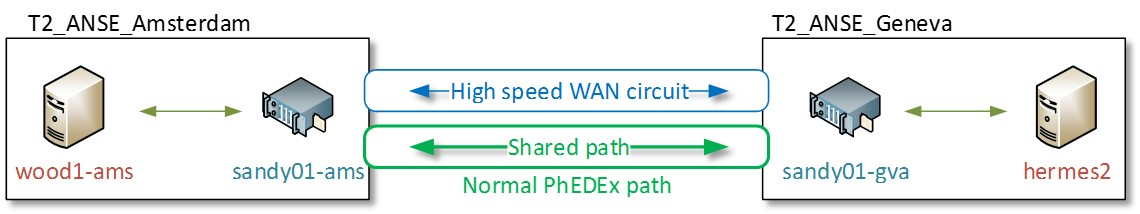
\includegraphics[width=0.95\textwidth]{Figures/FileDownload_ANSE_Testbed.jpg}
  \caption{PhEDEx testbed for ANSE}
  \label{fig:ANSE-setup}
\end{figure}

\subsection{Results}

The results are summarised in Figure \ref{fig:combined_transfers}. This plot portrays the transfer 
speeds that PhEDEx achieved in our test scenario. The left half of the plot shows the PhEDEx 
throughput in the first part of the test while it was competing with the iperf traffic. Naturally, 
this limits PhEDEx traffic to ~600MB/sec (~4800 Gbps). The right part of the plot, displays the 
transfer speeds PhEDEx achieved on an empty link, with no competing traffic. An effective doubling 
of throughput is seen, with PhEDEx being able to fill up the whole 10 Gbps link.
The seesaw look of this plot is linked to the fact that PhEDEx has a delay between finishing one job and 
starting the next. This is due to various factors: pre/post validation, preparation of copyjobs or 
even time spent by the backend itself before actually launching a transfer. Because of these delays, 
the average rates reported by PhEDEx (Figure \ref{fig:combined_phedex_transfers}) will always be lower 
than the average rates of each individual transfer job. 
Lastly, Figure \ref{fig:combined_transfers} also shows the fact that there was no interruption in service 
when PhEDEx moved from one link to another. This test demonstrates the potential usefulness of 
using virtual circuits in PhEDEx.

\begin{figure}[h]
  \centering
  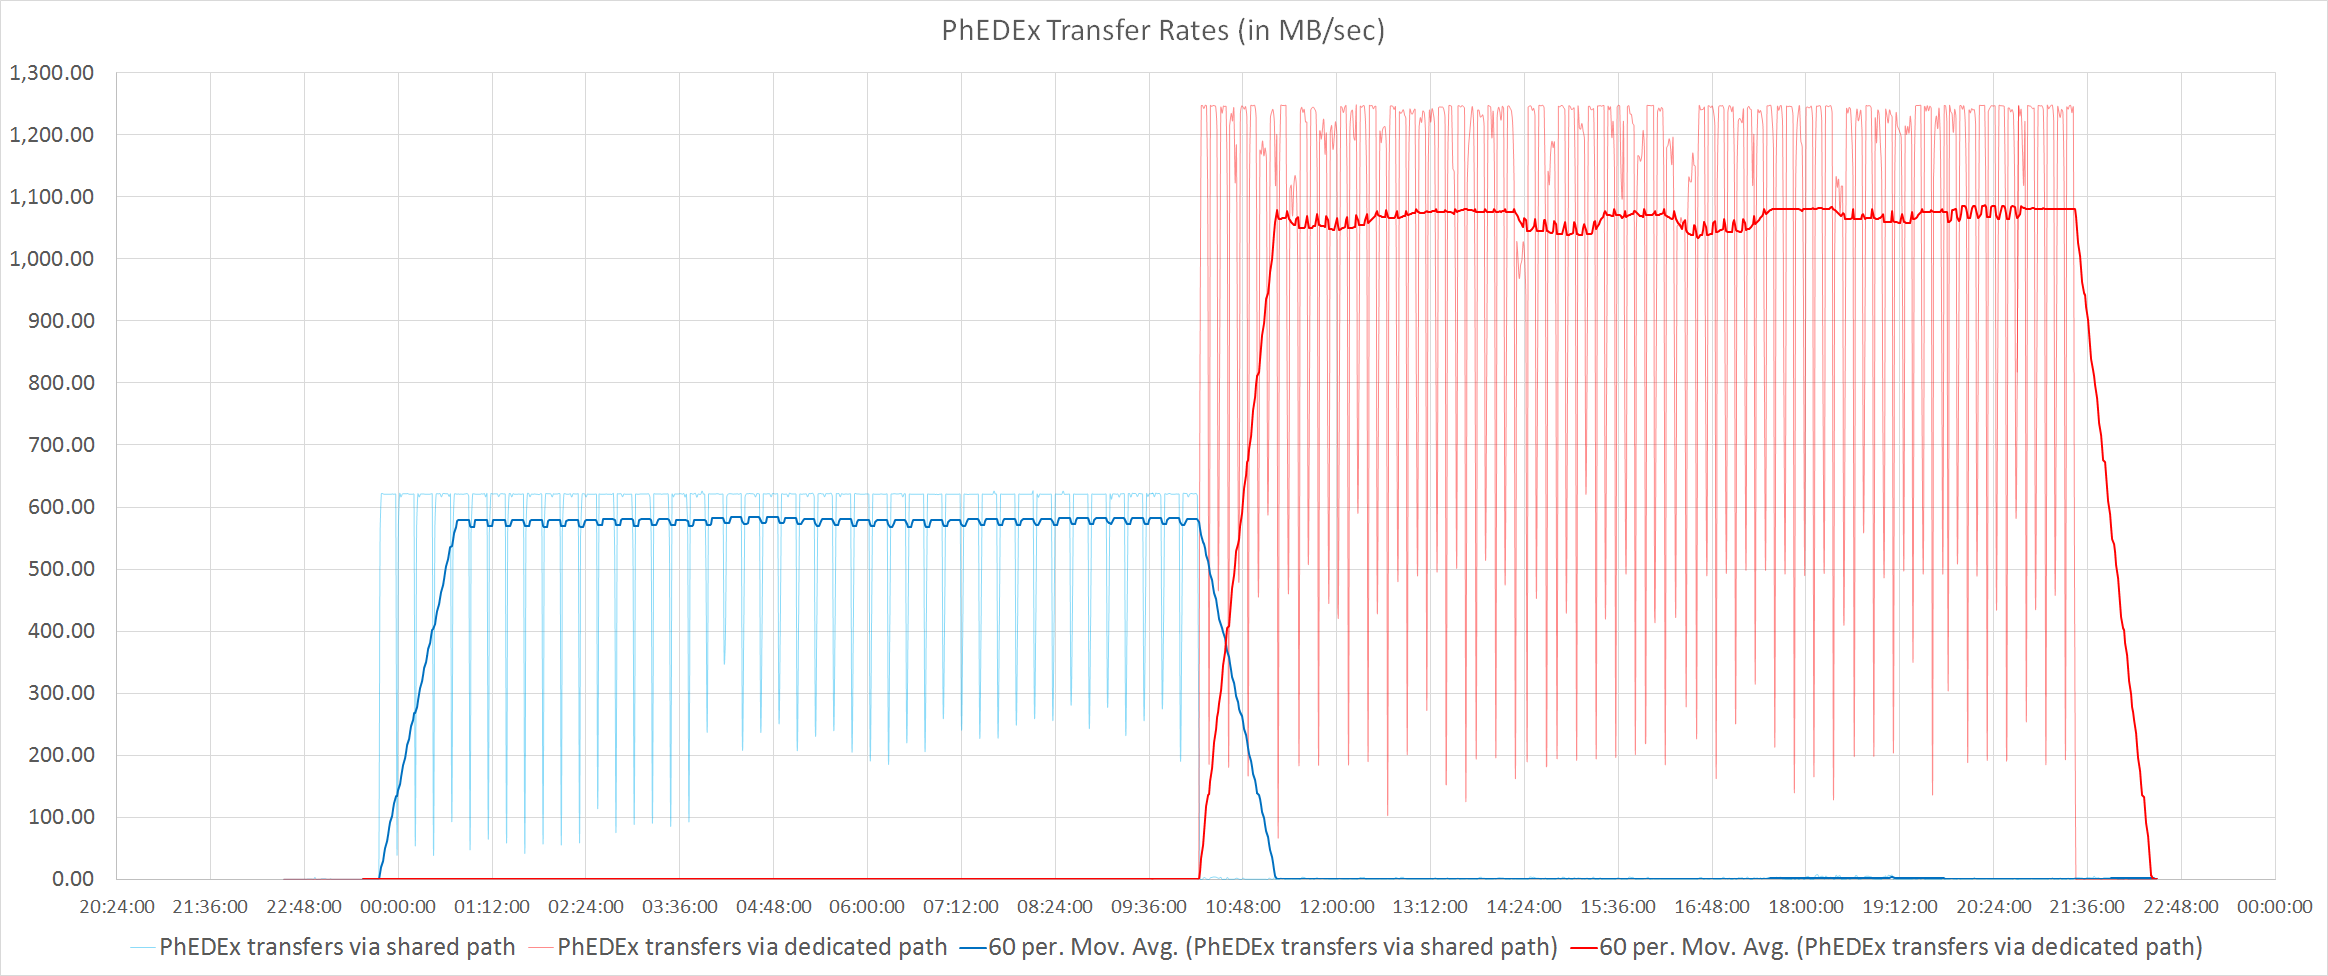
\includegraphics[width=0.95\textwidth]{Figures/FileDownload_All_paths.png}
  \caption{View of PhEDEx-only transfers on both the shared and dedicated path}
  \label{fig:combined_transfers}
\end{figure} 

\begin{figure}[h]
  \centering
  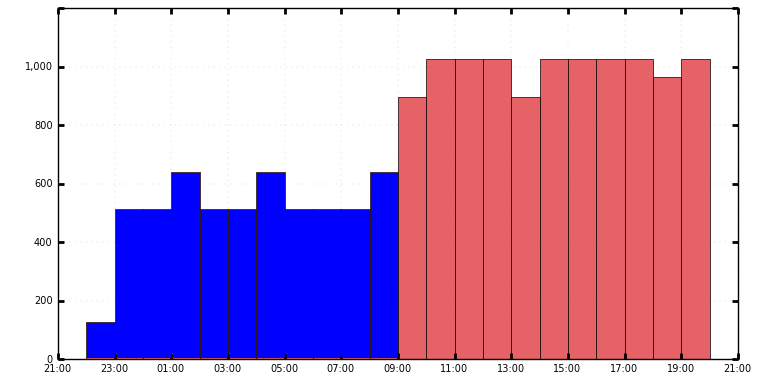
\includegraphics[width=0.95\textwidth]{Figures/FileDownload_PhEDEx_all_paths.png}
  \caption{View of PhEDEx only transfers on both the shared and dedicated path}
  \label{fig:combined_phedex_transfers}
\end{figure} 

\subsection{Prototype limitations}

The prototype proved helpful in demonstrating that circuits can be useful, and that circuit 
awareness can be integrated into PhEDEx, specifically at the site level. The design decisions 
taken in the development process mirror the need for a fast working prototype and this 
ultimately had an impact on its ultimate usefulness.

\begin{itemize}
  \item Non-modular design: All of the control logic was contained in the FileDownload agent.
  This meant that the part that requests circuits and manages their lifecycle could not be 
  separated from the FileDownload agent. This was needed in order to create a stand alone 
  application that could be used external tools as well.
  \item Single circuit backend: Relied on a single method of requesting circuits (DYNES). 
  For every different circuit provider used, a major change in code was required.
  \item Relied on FDT as a transfer tool: Unfortunately, this transfer tool is not widely used
  in production. Our production ready version should at least support the most common protocols
  out there (ie. FTS/SRM/gridFTP)
\end{itemize}

In addition to these decisions, it was assumed that a simple storage system would be used.
In all transfers involving the prototype, data was always moved from server to server, not 
from a storage farm to a storage farm. This becomes an issue when when extrapolating from a 
prototype to a production infrastructure since, it is assumed that the PFNs that PhEDEx 
receives, correspond to the actual location of files on a server. In this scenario, the 
endpoints of the circuits are known: the hostnames/IPs in a PFN correspond to a circuit 
endpoint.
In a transfer involving the storage farm, the PFN points to a server which then redirects 
to one of the replicas available. Until this redirection is done there is no way of knowing 
which servers will be involved in the transfer, therefore the endpoints of the circuit are 
unknown.